\documentclass{ximera}

\outcome{Compare and contrast local and absolute maxima and minima.}
\outcome{When can we guarantee an absolute maximum or minimum?}
\outcome{What is a critical point?}
\outcome{Find critical points.}
\outcome{Find the absolute max or min of a continuous function on a closed interval.}
\outcome{Solve basic word problems involving maxima or minima.}

\title{Maxima and minima}

\begin{document}

\begin{abstract}
  Derivatives can also help us identify local maxima and minima.
\end{abstract}
\maketitle


Whether we are interested in a function as a purely mathematical
object or in connection with some application to the real world, it is
often useful to know what the graph of the function looks like. We can
obtain a good picture of the graph using certain crucial information
provided by derivatives of the function and certain limits.

\section{Extrema}

Local \textit{extrema} on a function are points on the graph where the
$y$ coordinate is larger (or smaller) than all other $y$ coordinates
on the graph at points ``close to'' $(x,y)$. 

\begin{definition}\hfil
\begin{enumerate}
\item A point $(x,f(x))$ is a \textbf{local maximum} if there is an
  interval $a<x<b$ with $f(x)\ge f(z)$ for every $z$ in $(a,b)$.
\item A point $(x,f(x))$ is a \textbf{local minimum} if
  there is an interval $a<x<b$ with $f(x)\le f(z)$ for every $z$ in
  $(a,b)$.
\end{enumerate}
A \textbf{local extremum} is either a local maximum or a local
minimum.
\end{definition}

Local maximum and minimum points are quite distinctive on the graph of
a function, and are therefore useful in understanding the shape of the
graph. In many applied problems we want to find the largest or
smallest value that a function achieves (for example, we might want
to find the minimum cost at which some task can be performed) and so
identifying maximum and minimum points will be useful for applied
problems as well.

If $(x,f(x))$ is a point where $f(x)$ reaches a local maximum or
minimum, and if the derivative of $f$ exists at $x$, then the graph
has a tangent line and the tangent line must be horizontal. This is
important enough to state as a theorem, though we will not prove it.

\begin{theorem}[Fermat's Theorem]
If $f(x)$ has a local extremum at $x=a$ and $f(x)$ is differentiable
at $a$, then $f'(a)=0$.
\end{theorem}

\begin{image}
  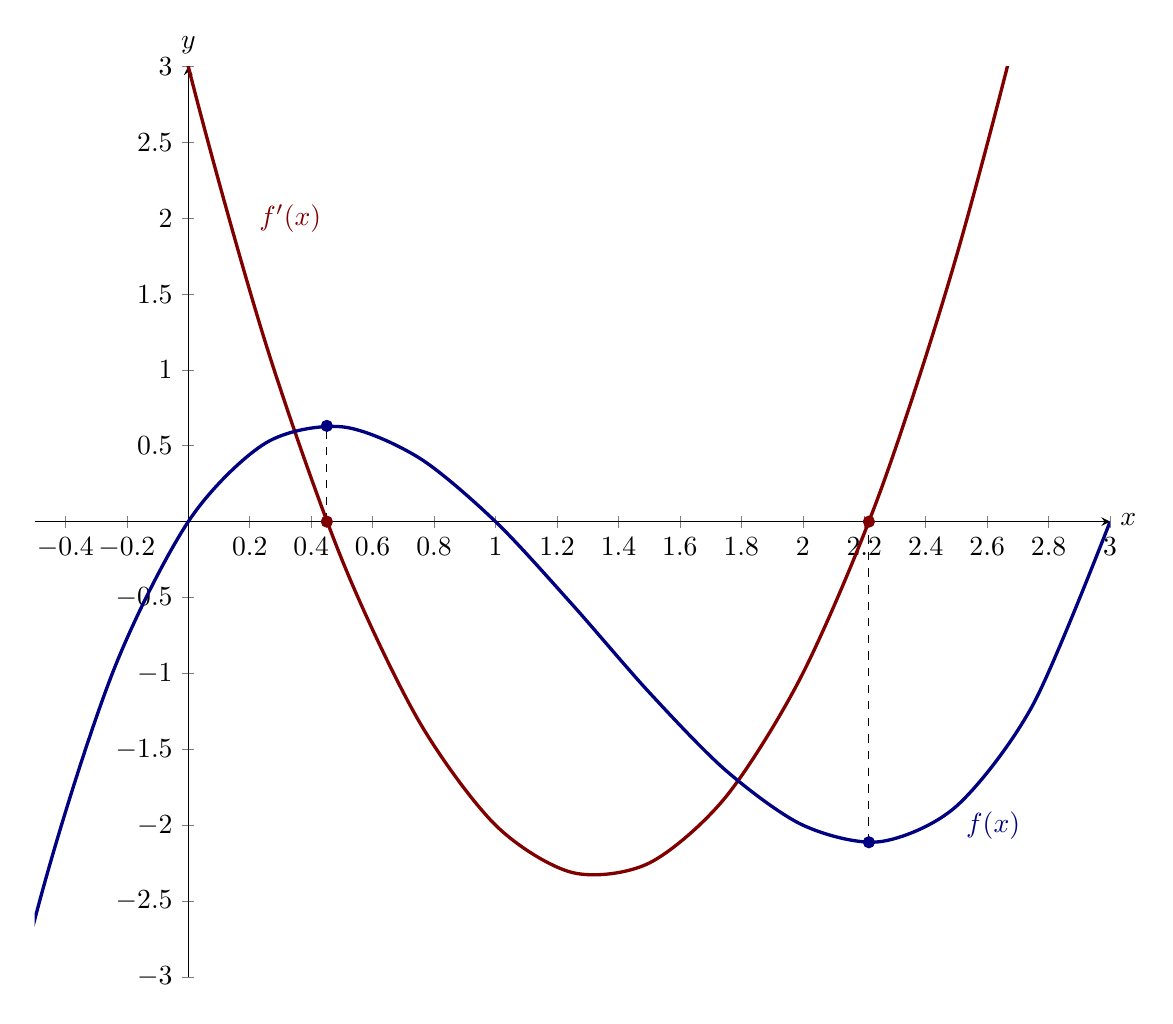
\begin{tikzpicture}
    \colorlet{textColor}{black}
    \colorlet{penColor2}{red!50!black}
    \colorlet{penColor}{blue!50!black}
	\begin{axis}[
            domain=-3:3,
            ymax=3,
            ymin=-3,
            width=6in,
            %samples=100,
            axis lines =middle, xlabel=$x$, ylabel=$y$,
            every axis y label/.style={at=(current axis.above origin),anchor=south},
            every axis x label/.style={at=(current axis.right of origin),anchor=west}
          ]
          \addplot [dashed, textColor, smooth] plot coordinates {(.451,0) (.451,.631)}; %% {.451};
          \addplot [dashed, textColor, smooth] plot coordinates {(2.215,-2.113) (2.215,0)}; %% axis{2.215};
          \addplot [very thick, penColor2, smooth] {3*x^2-8*x+3};
          \addplot [very thick, penColor, smooth] {x^3-4*x^2+3*x};
          \node at (axis cs:2.5,-2) [anchor=west] {\color{penColor}$f(x)$};  
          \node at (axis cs:.2,2) [anchor=west] {\color{penColor2}$f'(x)$};
          \addplot[color=penColor2,fill=penColor2,only marks,mark=*] coordinates{(.451,0)};  %% closed hole
          \addplot[color=penColor2,fill=penColor2,only marks,mark=*] coordinates{(2.215,0)};  %% closed hole
          \addplot[color=penColor,fill=penColor,only marks,mark=*] coordinates{(.451,.631)};  %% closed hole
          \addplot[color=penColor,fill=penColor,only marks,mark=*] coordinates{(2.215,-2.113)};  %% closed hole
        \end{axis}
\end{tikzpicture}
\end{image}
Thus, the only points at which a function can have a local maximum or
minimum are points at which the derivative is zero, see the above
image, or the derivative is undefined, as in the image below.
\begin{image}
\begin{tikzpicture}
    \colorlet{textColor}{black}
    \colorlet{penColor2}{red!50!black}
    \colorlet{penColor}{blue!50!black}
	\begin{axis}[
            width=6in,
            domain=-3:3,
            ymax=2,
            ymin=-2,
            axis lines =middle, xlabel=$x$, ylabel=$y$,
            every axis y label/.style={at=(current axis.above origin),anchor=south},
            every axis x label/.style={at=(current axis.right of origin),anchor=west}
          ]
          \addplot [very thick, penColor2, samples=100, smooth,domain=(-3:-.01)] {-(2/3)*abs(x)^(-1/3)};
          \addplot [very thick, penColor2, samples=100, smooth,domain=(.01:3)] {(2/3)*abs(x)^(-1/3)};
          \addplot [very thick, penColor, smooth,domain=(-3:-.01)] {abs(x)^(2/3)};
          \addplot [very thick, penColor, smooth,domain=(.01:3)] {x^(2/3)};         
          \node at (axis cs:-2,1.7) [anchor=west] {\color{penColor}$f(x)$};  
          \node at (axis cs:2,.7) [anchor=west] {\color{penColor2}$f'(x)$};
        \end{axis}
\end{tikzpicture}
\end{image}


\begin{definition}
Any value of $x$ for which $f'(x)$ is zero or undefined is called a
\textbf{critical point} for $f(x)$.
\end{definition}

\begin{warning} 
When looking for local maximum and minimum points, you are likely to
make two sorts of mistakes: 
\begin{itemize}
\item You may forget that a maximum or minimum can occur where the
  derivative does not exist, and so forget to check whether the
  derivative exists everywhere. 
\item You might assume that any place that the derivative is zero is a
  local maximum or minimum point, but this is not true, consider
  $y=x^3$.
\end{itemize}
\end{warning}

\begin{question}
  Critical points are values of $x$ where the derivative of the
  function equals zero.
    \begin{multipleChoice}
      \choice[correct]{False.}
      \choice{True.}
    \end{multipleChoice}    
\end{question}


\begin{question}
  Find the critical points of $x^3-12x^2+48x-64$.
    \begin{prompt}
      $x=$\answer{4}.
    \end{prompt}
\end{question}


\begin{question}
  Does $x^3-12x^2+48x-64$ have a local extrema at its critical point(s)?
    \begin{multipleChoice}
      \choice[correct]{No.}
      \choice{Yes.}
    \end{multipleChoice}
\end{question}

\begin{question}
  Does $x^3-3x^2-x+1$ have a local extrema at its critical point(s)?
    \begin{multipleChoice}
      \choice[correct]{Yes.}
      \choice{No.}
    \end{multipleChoice}
\end{question}

\begin{question}
Write down at least \textbf{five} questions for this lecture. After
you have your questions, label them as ``Level 1,'' ``Level 2,'' or
``Level 3'' where:
\begin{description}
\item[Level 1] Means you know the answer, or know exactly how to do this problem.
\item[Level 2] Means you think you know how to do the problem, or will
  soon learn how to do the problem.
\item[Level 3] Means you have no idea how to do the problem. 
\end{description}
  \begin{freeResponse}
  \end{freeResponse}
\end{question}

\end{document}
